\section{Day 3: Assignment Expectations, Heaps (Sept 8, 2025)}

The CLRS chapter on binomial heaps is posted on Quercus, because it was removed after the 2nd chapter.


\subsection{Assignment Expectations}

For reference, the solutions to Assignment 1 takes up roughly 4-5 pages. TLDR: Emulate the style of proof found in CLRS

\subsubsection*{Bounds}
\begin{itemize}
    \item Need to show upper and lower bound \textbf{separately}\footnote{note that no technique exists to directly show $\Theta$, without showing $O$ and $\Omega$ beforehand}
    \item To show $f(n) \in O(n)$ or $\Omega(n)$, we don't need to find specific values for $c, n_0$, just need to simplify $f$ such that it's clear 
\end{itemize}

\subsubsection*{Algorithms}
To give/describe an algorithm:
\begin{itemize}
\item Start with higher-level details, explain its phases
    \item Describe all parts of the algorithm in \textit{English}, which can easily be converted to pseudo-code. Don't miss edge cases, and pointer updates when the happen. Your peers should be able to understand it clearly.
    \item Producing pseudo-code is \textbf{optional}, unless explicitly asked for
    \item You can use algorithms you previously encountered in class or in past courses
    \item Diagrams are helpful, but cannot replace your English description
\end{itemize}

\subsubsection*{Proof of Correctness}
\begin{itemize}
    \item Always say what you are proving. For long results, introduce lemmas, for short results, that is unnecessary. No flow of consciousness!
    \item Make clear what proof technique you're using: ``We will prove by induction on the length $n$ \dots '', ``Suppose for contradiction that \dots''
    \item We can be less formal, we don't need to explicitly state what $P$ is, no CSC240-indentation is strictly required. Still use indentations to break up paragraphs though, for clarity.
\end{itemize}

\newpage
\subsection{Building Heaps}

We want an $\Theta(n)$ algorithm to make an array $A$ possess the MaxHeap property (in-place). 

\subsection*{BuildMaxHeap($A[1...n]$)}
\begin{algorithmic}[1]
\State A.heapsize = n
\For{$i = \lfloor \frac{n}{2} \rfloor$ to 1}
    \State MaxHeapify($A[i]$)
\EndFor
\end{algorithmic}
The loop invariant is that at the start of the iteration of the floor loop, $A[i+1]$, $\dots$, $A[n]$ is the root of a MaxHeap. 

At most $n$ calls will be made to the \textsc{MaxHeapify} function, each taking $O(\log n)$ steps in the worst case, meaning the total steps is $O(n \log n)$. This analysis isn't wrong per-se, it is a valid upper bound, just not a tight one.

The reason the bound wasn't tight is because for the lower levels, we are performing a lot less swaps than $\log n$. We observe that there are at most $2^{h - i}$ nodes at the $i$-th level (note that the root is considered to be at level 0). \textsc{MaxHeapify} on a node of height $i$ takes at most $ci$ steps.
\begin{align*}
    T(n) &= c \cdot \sum_{i=1}^{h} 2^{h-i} i \\
    &= c \cdot 2^h \sum_{i=1}^{h} \frac{i}{2^i} \\
    &\leq cn \sum_{i=1}^{\infty} \frac{i}{2^i} \\
    &= 2cn \in O(n)
\end{align*}

For the lower bound, at least $\lfloor \frac{n}{2} \rfloor$ calls to \textsc{MaxHeapify} are made, because of the loop terminatwith each taking at least 1 step. Hence it is $\Omega(n)$.

\subsection{Binomial Heaps}

We want \textit{mergeable} priority queues, which support an additional operation.
\begin{description}
    \item[Union($S_1, S_2$)] Given two priority queues $S_1$ and $S_2$, merge them into a single queue with the union of their elements. Assume the elements in $S_1$ and $S_2$ are disjoint. 
\end{description}

\begin{definition}[Binomial Trees]
A binomial tree of degree $k$ is defined recursively:
\begin{itemize} 
\item $B_0$ is a single node 
    \item $B_k$ consists of two binomial trees $B_{k-1}$, with the root of 1 being the leftmost child of the root of the other 
\end{itemize}
\end{definition}

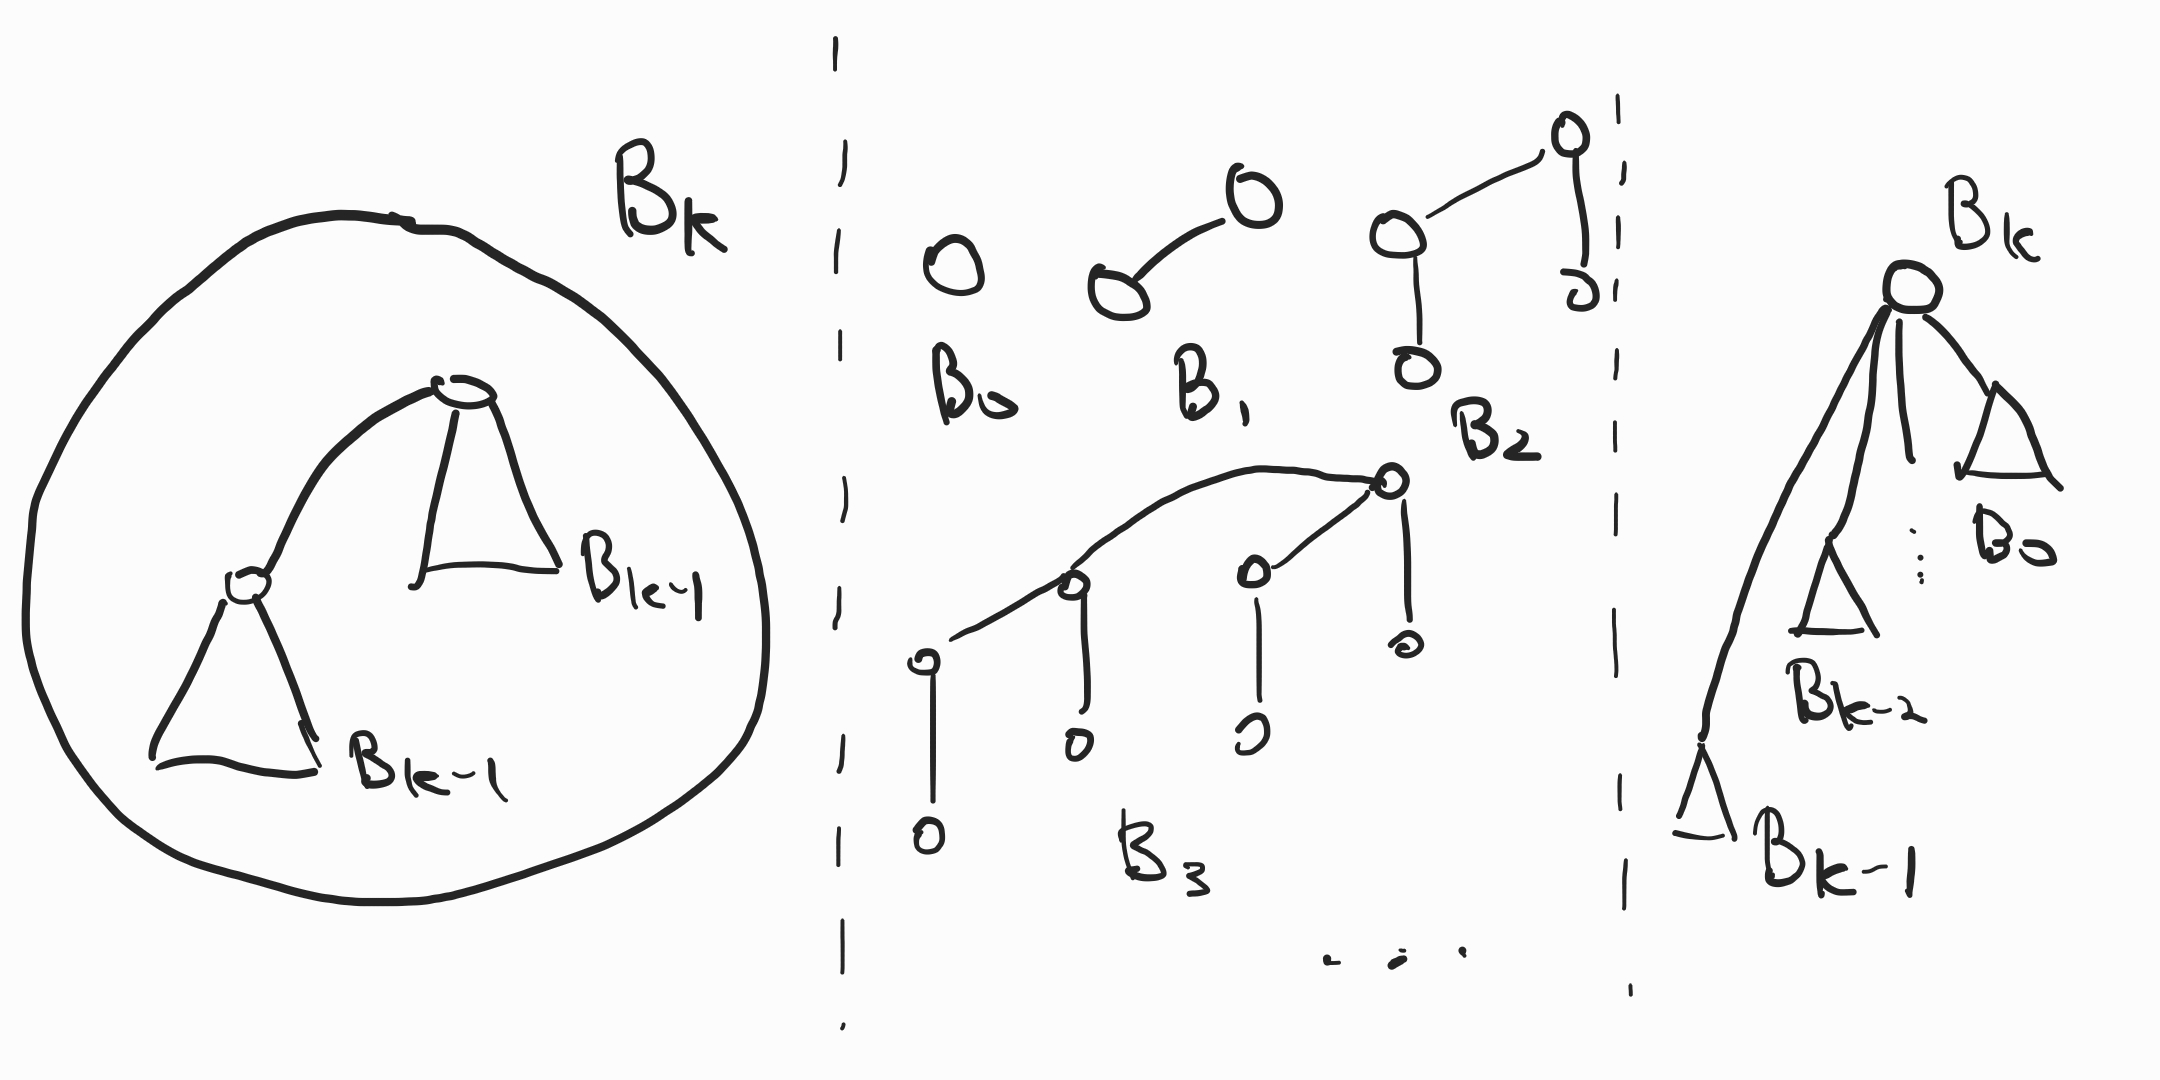
\includegraphics{csc265/figures/binomialtree.jpg}

\noindent For a binomial tree of degree $k$,
\begin{enumerate}
\item There are $2^k$ nodes
\item The height is $k$
    \item There are exactly $\binom{k}{i}$ nodes at depth $i$\footnote{follows from combinatorics facts}
    \item The root has degree $k$ and its $i$-th child is the root of a binomial tree $B_i$ (children are labelled $k-1$ to 0 left to right) 
\end{enumerate}

Defining the operations this way makes the operations quite simple, we didn't have time to go over them this class.
